\begin{Code}
romc.solve_problems(n1, use_bo = False, optimizer_args = None)
\end{Code}

\noindent
This method (a) draws the nuisance variables, (b) defines the
optimisation problems and (c) solves them using either a
gradient-based optimiser or the Bayesian optimisation (B0) scheme. The
three tasks are completed sequentially, as shown in
Figure~\ref{fig:romc_overview}. The definition of the optimisation
problems is performed by drawing \code{n1} integer numbers from a
discrete uniform distribution \(u_i \sim \mathcal{U}\{1,
2^{32}-1\}\). Each integer \(u_i\) is the seed used in \pkg{ELFI}'s
random simulator. The user may select the Bayesian Optimisation scheme
by setting the argument \code{use_bo = True} and pass custom arguments
to the optimizer through \code{optimize_args}.

\begin{Code}
romc.distance_hist(**kwargs)
\end{Code}

\noindent
This function helps the user decide which threshold \(\epsilon\) to
use, by plotting a histogram of the distances at the optimal point
\(d_i(\thetab_i^*) : \{i = 1, 2, \ldots, n_1\}\) or \(\hat{d}_i^*\) in
case \code{use_bo=True}. The function accepts all keyword arguments
and forwards them to the underlying \code{pyplot.hist()} function of
the package \pkg{matplotlib}. In this way the user may customise some
properties of the histogram, such as the number of bins or the range
of values.

\begin{Code}
romc.estimate_regions(eps_filter, use_surrogate=None, fit_models=False)
\end{Code}

\noindent
This method estimates the proposal region around the optimal points,
following Algorithm~\ref{alg:region_construction}. By default, the
distance model that will be used follows the decision from the
previous step; if a gradient-based optimizer has been used, then the
real distance function \(d\) will be chosen. If BO, then then the
surrogate model \(\hat{d}\). In case, the user wants to enforce using
the original distance function \(d\) after BO, they may set
\code{use_surrogate=False}. Finally, the option \code{fit_models}
defines whether to fit local surrogate models \(\tilde{d}\) after
estimating the proposal regions.

\begin{Code}
romc.fit_posterior(args*)  # training in a single call
romc.visualize_region(i)   # acceptance region
romc.compute_eps(quantile) # estimates eps
----------------------------------------------------------------------------
\end{Code}

\noindent
The function \code{fit_posterior} is a syntactic sugar for applying
\code{solve_problems} and \\ \code{estimate_regions} into a single
step. The function \code{visualize_region} can be used for plotting
the bounding box around the optimal point, when the parameter space is
up to 2D. The argument \code{i} is the index of the corresponding
optimisation problem. Finally, \code{compute_eps} returns the
appropriate distance value \(d_{i=\kappa}^*\) where
\(\kappa = \lfloor quantile \cdot n \rfloor\) from the collection
\(\{ d_i^* \} \forall i = \{1, \ldots, n\}\) where \(n\) is the number
of accepted solutions. It can be used to automate the selection of the
threshold \(\epsilon\), e.g.,
\code{eps=romc.compute_eps(quantile=0.9)}.


\subsubsection*{Example}


In the following snippet, we put together the routines described above
to perform the training part at our running example.

\begin{Code}
# Training (fitting) part
n1 = 500 # number of optimisation problems
seed = 21 # seed for solving the optimisation problems
use_bo = False # set to True for switching to Bayesian optimisation

# Training step-by-step
romc.solve_problems(n1 = n1, seed = seed, use_bo = use_bo)
romc.theta_hist(bins = 100) # plot hist to decide which eps to use

eps = .75 # threshold for the bounding box 
romc.estimate_regions(eps = eps) # build the bounding boxes

romc.visualize_region(i = 1) # for inspecting visually the bounding box

# Equivalent one-line command
# romc.fit_posterior(n1 = n1, eps = eps, use_bo = use_bo, seed = seed)
\end{Code}

\begin{figure}[ht]
  \begin{center}    
    % This file was created with tikzplotlib v0.9.12.
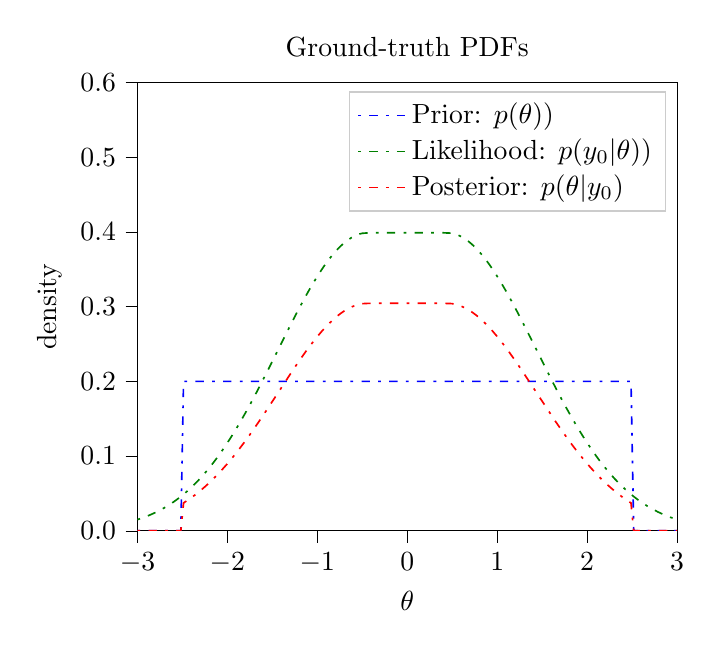
\begin{tikzpicture}

\begin{axis}[
legend cell align={left},
legend style={fill opacity=0.8, draw opacity=1, text opacity=1, draw=white!80!black},
tick align=outside,
tick pos=left,
title={Ground-truth PDFs},
x grid style={white!69.0196078431373!black},
xlabel={\(\displaystyle \theta\)},
xmin=-3, xmax=3,
xtick style={color=black},
xtick={-3,-2,-1,0,1,2,3},
xticklabels={
  \(\displaystyle {\ensuremath{-}3}\),
  \(\displaystyle {\ensuremath{-}2}\),
  \(\displaystyle {\ensuremath{-}1}\),
  \(\displaystyle {0}\),
  \(\displaystyle {1}\),
  \(\displaystyle {2}\),
  \(\displaystyle {3}\)
},
y grid style={white!69.0196078431373!black},
ylabel={density},
ymin=0, ymax=0.6,
ytick style={color=black},
ytick={0,0.1,0.2,0.3,0.4,0.5,0.6},
yticklabels={
  \(\displaystyle {0.0}\),
  \(\displaystyle {0.1}\),
  \(\displaystyle {0.2}\),
  \(\displaystyle {0.3}\),
  \(\displaystyle {0.4}\),
  \(\displaystyle {0.5}\),
  \(\displaystyle {0.6}\)
}
]
\addplot [semithick, blue, dash pattern=on 1pt off 3pt on 3pt off 3pt]
table {%
-3 0
-2.51758790016174 0
-2.48743724822998 0.200000047683716
2.48743724822998 0.200000047683716
2.51758790016174 0
3 0
};
\addlegendentry{Prior: $p(\theta))$}
\addplot [semithick, green!50!black, dash pattern=on 1pt off 3pt on 3pt off 3pt]
table {%
-3 0.0149635076522827
-2.9396984577179 0.0174322128295898
-2.87939691543579 0.0202344655990601
-2.81909537315369 0.0234019756317139
-2.75879406929016 0.0269670486450195
-2.69849252700806 0.030962347984314
-2.63819098472595 0.0354206562042236
-2.57788944244385 0.0403739213943481
-2.51758790016174 0.0458526611328125
-2.45728635787964 0.0518859624862671
-2.39698481559753 0.0584999322891235
-2.33668351173401 0.0657176971435547
-2.2763819694519 0.07355797290802
-2.2160804271698 0.082034707069397
-2.1557788848877 0.0911562442779541
-2.09547734260559 0.100924491882324
-2.03517580032349 0.111333727836609
-1.97487437725067 0.122370958328247
-1.91457283496857 0.134014010429382
-1.85427141189575 0.1462322473526
-1.79396986961365 0.158985257148743
-1.73366832733154 0.172223091125488
-1.67336678504944 0.185885906219482
-1.61306536197662 0.199904561042786
-1.52261304855347 0.221424460411072
-1.28140699863434 0.279423117637634
-1.22110557556152 0.293476581573486
-1.16080403327942 0.30711817741394
-1.10050249099731 0.320227146148682
-1.04020094871521 0.332683801651001
-0.979899525642395 0.344370484352112
-0.949748754501343 0.349889516830444
-0.919597983360291 0.355173826217651
-0.889447212219238 0.360210537910461
-0.859296560287476 0.364986658096313
-0.829145669937134 0.369489908218384
-0.798995018005371 0.373708963394165
-0.768844246864319 0.377632856369019
-0.738693475723267 0.381250977516174
-0.708542704582214 0.384554147720337
-0.678391933441162 0.38753342628479
-0.648241281509399 0.390181064605713
-0.618090391159058 0.392489671707153
-0.587939739227295 0.394453287124634
-0.557788968086243 0.396066427230835
-0.52763819694519 0.397324919700623
-0.497487425804138 0.398194551467896
-0.437186002731323 0.398676156997681
-0.346733689308167 0.398900628089905
-0.0150753259658813 0.398942232131958
0.407035112380981 0.398792028427124
0.467336654663086 0.398488640785217
0.497487425804138 0.398194551467896
0.52763819694519 0.397324919700623
0.557788968086243 0.396066427230835
0.587939739227295 0.394453287124634
0.618090391159058 0.392489671707153
0.648241281509399 0.390181064605713
0.678391933441162 0.38753342628479
0.708542704582214 0.384554147720337
0.738693475723267 0.381250977516174
0.768844246864319 0.377632856369019
0.798995018005371 0.373708963394165
0.829145669937134 0.369489908218384
0.859296560287476 0.364986658096313
0.889447212219238 0.360210537910461
0.919597983360291 0.355173826217651
0.949748754501343 0.349889516830444
0.979899525642395 0.344370484352112
1.04020094871521 0.332683801651001
1.10050249099731 0.320227146148682
1.16080403327942 0.30711817741394
1.22110557556152 0.293476581573486
1.28140699863434 0.279423117637634
1.3718593120575 0.257830619812012
1.58291459083557 0.207022905349731
1.64321613311768 0.192855477333069
1.70351755619049 0.17900550365448
1.7638190984726 0.165547132492065
1.8241206407547 0.152544856071472
1.88442206382751 0.140053510665894
1.94472360610962 0.128118515014648
2.00502514839172 0.116775035858154
2.06532669067383 0.106049656867981
2.12562823295593 0.0959596633911133
2.18592953681946 0.0865145921707153
2.24623107910156 0.0777161121368408
2.30653262138367 0.0695589780807495
2.36683416366577 0.0620321035385132
2.42713570594788 0.0551187992095947
2.48743724822998 0.0487983226776123
2.54773879051208 0.0430457592010498
2.60804009437561 0.0378334522247314
2.66834163665771 0.0331317186355591
2.72864317893982 0.0289088487625122
2.78894472122192 0.0251327753067017
2.84924626350403 0.0217704772949219
2.90954780578613 0.0187896490097046
2.96984934806824 0.0161581039428711
3 0.0149635076522827
};
\addlegendentry{Likelihood: $p(y_0|\theta))$}
\addplot [semithick, red, dash pattern=on 1pt off 3pt on 3pt off 3pt]
table {%
-3 0
-2.51758790016174 0
-2.48743724822998 0.0372545719146729
-2.42713570594788 0.0420799255371094
-2.36683416366577 0.0473577976226807
-2.30653262138367 0.0531041622161865
-2.24623107910156 0.0593316555023193
-2.18592953681946 0.0660487413406372
-2.12562823295593 0.0732594728469849
-2.06532669067383 0.0809625387191772
-2.00502514839172 0.0891507863998413
-1.94472360610962 0.0978107452392578
-1.88442206382751 0.106922507286072
-1.8241206407547 0.116458892822266
-1.7638190984726 0.12638533115387
-1.70351755619049 0.136659979820251
-1.61306536197662 0.152615189552307
-1.52261304855347 0.169044375419617
-1.25125622749329 0.21872091293335
-1.19095480442047 0.229304075241089
-1.13065326213837 0.239526867866516
-1.07035171985626 0.249297142028809
-1.01005029678345 0.258524179458618
-0.949748754501343 0.267119646072388
-0.889447212219238 0.274999141693115
-0.829145669937134 0.282083511352539
-0.798995018005371 0.285304546356201
-0.768844246864319 0.288300037384033
-0.738693475723267 0.291062355041504
-0.708542704582214 0.293584108352661
-0.678391933441162 0.29585862159729
-0.648241281509399 0.297879934310913
-0.618090391159058 0.299642443656921
-0.587939739227295 0.301141500473022
-0.557788968086243 0.302373051643372
-0.52763819694519 0.303333759307861
-0.497487425804138 0.303997755050659
-0.437186002731323 0.304365396499634
-0.316582918167114 0.304553270339966
0.346733689308167 0.304536819458008
0.467336654663086 0.304222345352173
0.497487425804138 0.303997755050659
0.52763819694519 0.303333759307861
0.557788968086243 0.302373051643372
0.587939739227295 0.301141500473022
0.618090391159058 0.299642443656921
0.648241281509399 0.297879934310913
0.678391933441162 0.29585862159729
0.708542704582214 0.293584108352661
0.738693475723267 0.291062355041504
0.768844246864319 0.288300037384033
0.798995018005371 0.285304546356201
0.829145669937134 0.282083511352539
0.889447212219238 0.274999141693115
0.949748754501343 0.267119646072388
1.01005029678345 0.258524179458618
1.07035171985626 0.249297142028809
1.13065326213837 0.239526867866516
1.19095480442047 0.229304075241089
1.25125622749329 0.21872091293335
1.34170854091644 0.202370405197144
1.64321613311768 0.147233605384827
1.73366832733154 0.131482005119324
1.79396986961365 0.121375799179077
1.85427141189575 0.111639618873596
1.91457283496857 0.102311730384827
1.97487437725067 0.0934228897094727
2.03517580032349 0.0849967002868652
2.09547734260559 0.077049732208252
2.1557788848877 0.0695923566818237
2.2160804271698 0.0626286268234253
2.2763819694519 0.056157112121582
2.33668351173401 0.0501714944839478
2.39698481559753 0.044661283493042
2.45728635787964 0.03961181640625
2.48743724822998 0.0372545719146729
2.51758790016174 0
3 0
};
\addlegendentry{Posterior: $p(\theta|y_0)$}
\end{axis}

\end{tikzpicture}

    % This file was created with tikzplotlib v0.9.12.
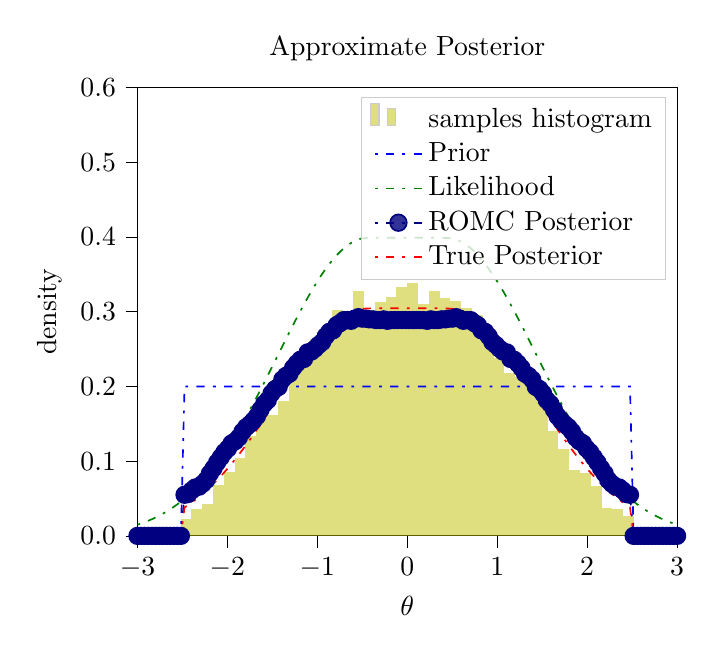
\begin{tikzpicture}

\definecolor{color0}{rgb}{0.75,0.75,0}

\begin{axis}[
legend cell align={left},
legend style={fill opacity=0.8, draw opacity=1, text opacity=1, draw=white!80!black},
tick align=outside,
tick pos=left,
title={Approximate Posterior},
x grid style={white!69.0196078431373!black},
xlabel={\(\displaystyle \theta\)},
xmin=-3, xmax=3,
xtick style={color=black},
xtick={-3,-2,-1,0,1,2,3},
xticklabels={
  \(\displaystyle {\ensuremath{-}3}\),
  \(\displaystyle {\ensuremath{-}2}\),
  \(\displaystyle {\ensuremath{-}1}\),
  \(\displaystyle {0}\),
  \(\displaystyle {1}\),
  \(\displaystyle {2}\),
  \(\displaystyle {3}\)
},
y grid style={white!69.0196078431373!black},
ylabel={density},
ymin=0, ymax=0.6,
ytick style={color=black},
ytick={0,0.1,0.2,0.3,0.4,0.5,0.6},
yticklabels={
  \(\displaystyle {0.0}\),
  \(\displaystyle {0.1}\),
  \(\displaystyle {0.2}\),
  \(\displaystyle {0.3}\),
  \(\displaystyle {0.4}\),
  \(\displaystyle {0.5}\),
  \(\displaystyle {0.6}\)
}
]
\draw[draw=none,fill=color0,fill opacity=0.5] (axis cs:-3,0) rectangle (axis cs:-2.88,0);
\addlegendimage{ybar,ybar legend,draw=none,fill=color0,fill opacity=0.5}
\addlegendentry{samples histogram}

\draw[draw=none,fill=color0,fill opacity=0.5] (axis cs:-2.88,0) rectangle (axis cs:-2.76,0);
\draw[draw=none,fill=color0,fill opacity=0.5] (axis cs:-2.76,0) rectangle (axis cs:-2.64,0);
\draw[draw=none,fill=color0,fill opacity=0.5] (axis cs:-2.64,0) rectangle (axis cs:-2.52,0);
\draw[draw=none,fill=color0,fill opacity=0.5] (axis cs:-2.52,0) rectangle (axis cs:-2.4,0.0231223039678857);
\draw[draw=none,fill=color0,fill opacity=0.5] (axis cs:-2.4,0) rectangle (axis cs:-2.28,0.0357920595667274);
\draw[draw=none,fill=color0,fill opacity=0.5] (axis cs:-2.28,0) rectangle (axis cs:-2.16,0.0432891657931185);
\draw[draw=none,fill=color0,fill opacity=0.5] (axis cs:-2.16,0) rectangle (axis cs:-2.04,0.0678278797971952);
\draw[draw=none,fill=color0,fill opacity=0.5] (axis cs:-2.04,0) rectangle (axis cs:-1.92,0.0853063510438926);
\draw[draw=none,fill=color0,fill opacity=0.5] (axis cs:-1.92,0) rectangle (axis cs:-1.8,0.104059662822912);
\draw[draw=none,fill=color0,fill opacity=0.5] (axis cs:-1.8,0) rectangle (axis cs:-1.68,0.133237638068697);
\draw[draw=none,fill=color0,fill opacity=0.5] (axis cs:-1.68,0) rectangle (axis cs:-1.56,0.164674290398949);
\draw[draw=none,fill=color0,fill opacity=0.5] (axis cs:-1.56,0) rectangle (axis cs:-1.44,0.161302362215871);
\draw[draw=none,fill=color0,fill opacity=0.5] (axis cs:-1.44,0) rectangle (axis cs:-1.32,0.180069616446029);
\draw[draw=none,fill=color0,fill opacity=0.5] (axis cs:-1.32,0) rectangle (axis cs:-1.2,0.221053630317552);
\draw[draw=none,fill=color0,fill opacity=0.5] (axis cs:-1.2,0) rectangle (axis cs:-1.08,0.246178284768201);
\draw[draw=none,fill=color0,fill opacity=0.5] (axis cs:-1.08,0) rectangle (axis cs:-0.96,0.262860963803752);
\draw[draw=none,fill=color0,fill opacity=0.5] (axis cs:-0.96,0) rectangle (axis cs:-0.84,0.276028000159873);
\draw[draw=none,fill=color0,fill opacity=0.5] (axis cs:-0.84,0) rectangle (axis cs:-0.72,0.302242310791823);
\draw[draw=none,fill=color0,fill opacity=0.5] (axis cs:-0.72,0) rectangle (axis cs:-0.6,0.290784833444551);
\draw[draw=none,fill=color0,fill opacity=0.5] (axis cs:-0.6,0) rectangle (axis cs:-0.48,0.328299321975026);
\draw[draw=none,fill=color0,fill opacity=0.5] (axis cs:-0.48,0) rectangle (axis cs:-0.36,0.302643424386121);
\draw[draw=none,fill=color0,fill opacity=0.5] (axis cs:-0.36,0) rectangle (axis cs:-0.24,0.313647235823262);
\draw[draw=none,fill=color0,fill opacity=0.5] (axis cs:-0.24,0) rectangle (axis cs:-0.12,0.319481615376679);
\draw[draw=none,fill=color0,fill opacity=0.5] (axis cs:-0.12,0) rectangle (axis cs:0,0.333217074740762);
\draw[draw=none,fill=color0,fill opacity=0.5] (axis cs:0,0) rectangle (axis cs:0.12,0.337997190488845);
\draw[draw=none,fill=color0,fill opacity=0.5] (axis cs:0.12,0) rectangle (axis cs:0.24,0.31078331335988);
\draw[draw=none,fill=color0,fill opacity=0.5] (axis cs:0.24,0) rectangle (axis cs:0.36,0.327787026270366);
\draw[draw=none,fill=color0,fill opacity=0.5] (axis cs:0.36,0) rectangle (axis cs:0.48,0.318103100207685);
\draw[draw=none,fill=color0,fill opacity=0.5] (axis cs:0.48,0) rectangle (axis cs:0.6,0.314153811547969);
\draw[draw=none,fill=color0,fill opacity=0.5] (axis cs:0.6,0) rectangle (axis cs:0.72,0.305401169721601);
\draw[draw=none,fill=color0,fill opacity=0.5] (axis cs:0.72,0) rectangle (axis cs:0.84,0.294962921302443);
\draw[draw=none,fill=color0,fill opacity=0.5] (axis cs:0.84,0) rectangle (axis cs:0.96,0.270674813920115);
\draw[draw=none,fill=color0,fill opacity=0.5] (axis cs:0.96,0) rectangle (axis cs:1.08,0.237704134465861);
\draw[draw=none,fill=color0,fill opacity=0.5] (axis cs:1.08,0) rectangle (axis cs:1.2,0.217649527247231);
\draw[draw=none,fill=color0,fill opacity=0.5] (axis cs:1.2,0) rectangle (axis cs:1.32,0.213227625243787);
\draw[draw=none,fill=color0,fill opacity=0.5] (axis cs:1.32,0) rectangle (axis cs:1.44,0.206217074812262);
\draw[draw=none,fill=color0,fill opacity=0.5] (axis cs:1.44,0) rectangle (axis cs:1.56,0.187841996707722);
\draw[draw=none,fill=color0,fill opacity=0.5] (axis cs:1.56,0) rectangle (axis cs:1.68,0.140157026319701);
\draw[draw=none,fill=color0,fill opacity=0.5] (axis cs:1.68,0) rectangle (axis cs:1.8,0.116292197453994);
\draw[draw=none,fill=color0,fill opacity=0.5] (axis cs:1.8,0) rectangle (axis cs:1.92,0.0886021319938282);
\draw[draw=none,fill=color0,fill opacity=0.5] (axis cs:1.92,0) rectangle (axis cs:2.04,0.0841287501707948);
\draw[draw=none,fill=color0,fill opacity=0.5] (axis cs:2.04,0) rectangle (axis cs:2.16,0.0663943098211411);
\draw[draw=none,fill=color0,fill opacity=0.5] (axis cs:2.16,0) rectangle (axis cs:2.28,0.0377386402449356);
\draw[draw=none,fill=color0,fill opacity=0.5] (axis cs:2.28,0) rectangle (axis cs:2.4,0.0361088034566983);
\draw[draw=none,fill=color0,fill opacity=0.5] (axis cs:2.4,0) rectangle (axis cs:2.52,0.0262897428675961);
\draw[draw=none,fill=color0,fill opacity=0.5] (axis cs:2.52,0) rectangle (axis cs:2.64,0);
\draw[draw=none,fill=color0,fill opacity=0.5] (axis cs:2.64,0) rectangle (axis cs:2.76,0);
\draw[draw=none,fill=color0,fill opacity=0.5] (axis cs:2.76,0) rectangle (axis cs:2.88,0);
\draw[draw=none,fill=color0,fill opacity=0.5] (axis cs:2.88,0) rectangle (axis cs:3,0);
\addplot [semithick, blue, dash pattern=on 1pt off 3pt on 3pt off 3pt]
table {%
-3 0
-2.95973154362416 0
-2.91946308724832 0
-2.87919463087248 0
-2.83892617449664 0
-2.79865771812081 0
-2.75838926174497 0
-2.71812080536913 0
-2.67785234899329 0
-2.63758389261745 0
-2.59731543624161 0
-2.55704697986577 0
-2.51677852348993 0
-2.47651006711409 0.2
-2.43624161073825 0.2
-2.39597315436242 0.2
-2.35570469798658 0.2
-2.31543624161074 0.2
-2.2751677852349 0.2
-2.23489932885906 0.2
-2.19463087248322 0.2
-2.15436241610738 0.2
-2.11409395973154 0.2
-2.0738255033557 0.2
-2.03355704697987 0.2
-1.99328859060403 0.2
-1.95302013422819 0.2
-1.91275167785235 0.2
-1.87248322147651 0.2
-1.83221476510067 0.2
-1.79194630872483 0.2
-1.75167785234899 0.2
-1.71140939597315 0.2
-1.67114093959732 0.2
-1.63087248322148 0.2
-1.59060402684564 0.2
-1.5503355704698 0.2
-1.51006711409396 0.2
-1.46979865771812 0.2
-1.42953020134228 0.2
-1.38926174496644 0.2
-1.3489932885906 0.2
-1.30872483221477 0.2
-1.26845637583893 0.2
-1.22818791946309 0.2
-1.18791946308725 0.2
-1.14765100671141 0.2
-1.10738255033557 0.2
-1.06711409395973 0.2
-1.02684563758389 0.2
-0.986577181208054 0.2
-0.946308724832215 0.2
-0.906040268456376 0.2
-0.865771812080537 0.2
-0.825503355704698 0.2
-0.785234899328859 0.2
-0.74496644295302 0.2
-0.704697986577181 0.2
-0.664429530201343 0.2
-0.624161073825503 0.2
-0.583892617449664 0.2
-0.543624161073826 0.2
-0.503355704697987 0.2
-0.463087248322148 0.2
-0.422818791946309 0.2
-0.38255033557047 0.2
-0.342281879194631 0.2
-0.302013422818792 0.2
-0.261744966442953 0.2
-0.221476510067114 0.2
-0.181208053691275 0.2
-0.140939597315437 0.2
-0.100671140939598 0.2
-0.0604026845637584 0.2
-0.0201342281879198 0.2
0.0201342281879193 0.2
0.0604026845637584 0.2
0.100671140939597 0.2
0.140939597315436 0.2
0.181208053691275 0.2
0.221476510067114 0.2
0.261744966442953 0.2
0.302013422818792 0.2
0.342281879194631 0.2
0.382550335570469 0.2
0.422818791946308 0.2
0.463087248322148 0.2
0.503355704697986 0.2
0.543624161073825 0.2
0.583892617449664 0.2
0.624161073825503 0.2
0.664429530201342 0.2
0.704697986577181 0.2
0.74496644295302 0.2
0.785234899328859 0.2
0.825503355704698 0.2
0.865771812080537 0.2
0.906040268456376 0.2
0.946308724832214 0.2
0.986577181208053 0.2
1.02684563758389 0.2
1.06711409395973 0.2
1.10738255033557 0.2
1.14765100671141 0.2
1.18791946308725 0.2
1.22818791946309 0.2
1.26845637583893 0.2
1.30872483221476 0.2
1.3489932885906 0.2
1.38926174496644 0.2
1.42953020134228 0.2
1.46979865771812 0.2
1.51006711409396 0.2
1.5503355704698 0.2
1.59060402684564 0.2
1.63087248322148 0.2
1.67114093959731 0.2
1.71140939597315 0.2
1.75167785234899 0.2
1.79194630872483 0.2
1.83221476510067 0.2
1.87248322147651 0.2
1.91275167785235 0.2
1.95302013422819 0.2
1.99328859060403 0.2
2.03355704697987 0.2
2.0738255033557 0.2
2.11409395973154 0.2
2.15436241610738 0.2
2.19463087248322 0.2
2.23489932885906 0.2
2.2751677852349 0.2
2.31543624161074 0.2
2.35570469798658 0.2
2.39597315436242 0.2
2.43624161073825 0.2
2.47651006711409 0.2
2.51677852348993 0
2.55704697986577 0
2.59731543624161 0
2.63758389261745 0
2.67785234899329 0
2.71812080536913 0
2.75838926174497 0
2.7986577181208 0
2.83892617449664 0
2.87919463087248 0
2.91946308724832 0
2.95973154362416 0
3 0
};
\addlegendentry{Prior}
\addplot [semithick, green!50!black, dash pattern=on 1pt off 3pt on 3pt off 3pt]
table {%
-3 0.0149634957859139
-2.95973154362416 0.0165765785104069
-2.91946308724832 0.0183338002156055
-2.87919463087248 0.0202444445066368
-2.83892617449664 0.0223179862127286
-2.79865771812081 0.0245640467794704
-2.75838926174497 0.0269923438082632
-2.71812080536913 0.0296126346587464
-2.67785234899329 0.0324346540920591
-2.63758389261745 0.0354680460013991
-2.59731543624161 0.0387222893510991
-2.55704697986577 0.0422066185257928
-2.51677852348993 0.0459299383765193
-2.47651006711409 0.049900734339975
-2.43624161073825 0.0541269780995744
-2.39597315436242 0.0586160293514222
-2.35570469798658 0.0633745343334427
-2.31543624161074 0.0684083218704037
-2.2751677852349 0.0737222977798975
-2.23489932885906 0.0793203385729367
-2.19463087248322 0.0852051854660348
-2.15436241610738 0.0913783397977739
-2.11409395973154 0.0978399610102198
-2.0738255033557 0.104588768412427
-2.03355704697987 0.111621947988045
-1.99328859060403 0.11893506554012
-1.95302013422819 0.126521987482169
-1.91275167785235 0.134374810584119
-1.87248322147651 0.142483801963751
-1.83221476510067 0.150837350577857
-1.79194630872483 0.159421931411866
-1.75167785234899 0.168222083491765
-1.71140939597315 0.177220402747788
-1.67114093959732 0.186397550645663
-1.63087248322148 0.195732279368967
-1.59060402684564 0.205201474186111
-1.5503355704698 0.214780213469083
-1.51006711409396 0.224441846649815
-1.46979865771812 0.234158090205974
-1.42953020134228 0.243899141563262
-1.38926174496644 0.253633810588603
-1.3489932885906 0.263329668130575
-1.30872483221477 0.272953210843248
-1.26845637583893 0.282470041310282
-1.22818791946309 0.291845062271088
-1.18791946308725 0.301042683543393
-1.14765100671141 0.310027040040042
-1.10738255033557 0.318762219095587
-1.06711409395973 0.327212495153405
-1.02684563758389 0.335342569719669
-0.986577181208054 0.343117814369326
-0.946308724832215 0.350504514493653
-0.906040268456376 0.357470111411221
-0.865771812080537 0.36398344042577
-0.825503355704698 0.370014962406976
-0.785234899328859 0.375536986494055
-0.74496644295302 0.380523881578029
-0.704697986577181 0.38495227430593
-0.664429530201343 0.388801231468594
-0.624161073825503 0.392052424781739
-0.583892617449664 0.394690276245891
-0.543624161073826 0.396702082472345
-0.503355704697987 0.398078116586891
-0.463087248322148 0.398520629493419
-0.422818791946309 0.39873857459125
-0.38255033557047 0.398850797702491
-0.342281879194631 0.398904702642417
-0.302013422818792 0.398928473935743
-0.261744966442953 0.398937885952852
-0.221476510067114 0.398941125617285
-0.181208053691275 0.398942048501881
-0.140939597315437 0.398942249345522
-0.100671140939598 0.398942278297073
-0.0604026845637584 0.398942280366088
-0.0201342281879198 0.398942280401427
0.0201342281879193 0.398942280401427
0.0604026845637584 0.398942280366088
0.100671140939597 0.398942278297073
0.140939597315436 0.398942249345522
0.181208053691275 0.398942048501881
0.221476510067114 0.398941125617285
0.261744966442953 0.398937885952852
0.302013422818792 0.398928473935743
0.342281879194631 0.398904702642417
0.382550335570469 0.398850797702491
0.422818791946308 0.39873857459125
0.463087248322148 0.398520629493419
0.503355704697986 0.398078116586891
0.543624161073825 0.396702082472345
0.583892617449664 0.394690276245891
0.624161073825503 0.392052424781739
0.664429530201342 0.388801231468594
0.704697986577181 0.38495227430593
0.74496644295302 0.380523881578029
0.785234899328859 0.375536986494055
0.825503355704698 0.370014962406976
0.865771812080537 0.36398344042577
0.906040268456376 0.357470111411221
0.946308724832214 0.350504514493653
0.986577181208053 0.343117814369326
1.02684563758389 0.335342569719669
1.06711409395973 0.327212495153405
1.10738255033557 0.318762219095588
1.14765100671141 0.310027040040042
1.18791946308725 0.301042683543393
1.22818791946309 0.291845062271088
1.26845637583893 0.282470041310283
1.30872483221476 0.272953210843248
1.3489932885906 0.263329668130575
1.38926174496644 0.253633810588603
1.42953020134228 0.243899141563263
1.46979865771812 0.234158090205974
1.51006711409396 0.224441846649815
1.5503355704698 0.214780213469083
1.59060402684564 0.205201474186111
1.63087248322148 0.195732279368967
1.67114093959731 0.186397550645663
1.71140939597315 0.177220402747788
1.75167785234899 0.168222083491765
1.79194630872483 0.159421931411866
1.83221476510067 0.150837350577857
1.87248322147651 0.142483801963751
1.91275167785235 0.134374810584119
1.95302013422819 0.12652198748217
1.99328859060403 0.11893506554012
2.03355704697987 0.111621947988045
2.0738255033557 0.104588768412427
2.11409395973154 0.0978399610102198
2.15436241610738 0.0913783397977739
2.19463087248322 0.0852051854660349
2.23489932885906 0.0793203385729367
2.2751677852349 0.0737222977798976
2.31543624161074 0.0684083218704039
2.35570469798658 0.0633745343334427
2.39597315436242 0.0586160293514222
2.43624161073825 0.0541269780995745
2.47651006711409 0.049900734339975
2.51677852348993 0.0459299383765193
2.55704697986577 0.0422066185257928
2.59731543624161 0.0387222893510992
2.63758389261745 0.0354680460013991
2.67785234899329 0.0324346540920591
2.71812080536913 0.0296126346587465
2.75838926174497 0.0269923438082632
2.7986577181208 0.0245640467794704
2.83892617449664 0.0223179862127286
2.87919463087248 0.0202444445066368
2.91946308724832 0.0183338002156055
2.95973154362416 0.0165765785104069
3 0.0149634957859139
};
\addlegendentry{Likelihood}
\addplot [semithick, blue!50.1960784313725!black, dash pattern=on 1pt off 3pt on 3pt off 3pt, mark=*, mark size=3, mark options={solid}]
table {%
-3 0
-2.95973154362416 0
-2.91946308724832 0
-2.87919463087248 0
-2.83892617449664 0
-2.79865771812081 0
-2.75838926174497 0
-2.71812080536913 0
-2.67785234899329 0
-2.63758389261745 0
-2.59731543624161 0
-2.55704697986577 0
-2.51677852348993 0
-2.47651006711409 0.0550098231827112
-2.43624161073825 0.055992141453831
-2.39597315436242 0.0609037328094303
-2.35570469798658 0.0648330058939096
-2.31543624161074 0.0658153241650295
-2.2751677852349 0.0697445972495088
-2.23489932885906 0.0746561886051081
-2.19463087248322 0.0834970530451866
-2.15436241610738 0.0903732809430255
-2.11409395973154 0.0982318271119843
-2.0738255033557 0.105108055009823
-2.03355704697987 0.111984282907662
-1.99328859060403 0.116895874263261
-1.95302013422819 0.1237721021611
-1.91275167785235 0.12671905697446
-1.87248322147651 0.131630648330059
-1.83221476510067 0.139489194499018
-1.79194630872483 0.145383104125737
-1.75167785234899 0.149312377210216
-1.71140939597315 0.154223968565815
-1.67114093959732 0.160117878192534
-1.63087248322148 0.168958742632613
-1.59060402684564 0.176817288801572
-1.5503355704698 0.181728880157171
-1.51006711409396 0.19056974459725
-1.46979865771812 0.196463654223969
-1.42953020134228 0.199410609037328
-1.38926174496644 0.209233791748527
-1.3489932885906 0.214145383104126
-1.30872483221477 0.217092337917485
-1.26845637583893 0.224950884086444
-1.22818791946309 0.230844793713163
-1.18791946308725 0.235756385068762
-1.14765100671141 0.236738703339882
-1.10738255033557 0.245579567779961
-1.06711409395973 0.246561886051081
-1.02684563758389 0.25049115913556
-0.986577181208054 0.255402750491159
-0.946308724832215 0.259332023575639
-0.906040268456376 0.267190569744597
-0.865771812080537 0.273084479371316
-0.825503355704698 0.275049115913556
-0.785234899328859 0.281925343811395
-0.74496644295302 0.284872298624754
-0.704697986577181 0.288801571709234
-0.664429530201343 0.288801571709234
-0.624161073825503 0.287819253438114
-0.583892617449664 0.290766208251473
-0.543624161073826 0.292730844793713
-0.503355704697987 0.290766208251473
-0.463087248322148 0.290766208251473
-0.422818791946309 0.289783889980354
-0.38255033557047 0.289783889980354
-0.342281879194631 0.288801571709234
-0.302013422818792 0.288801571709234
-0.261744966442953 0.289783889980354
-0.221476510067114 0.287819253438114
-0.181208053691275 0.288801571709234
-0.140939597315437 0.288801571709234
-0.100671140939598 0.288801571709234
-0.0604026845637584 0.288801571709234
-0.0201342281879198 0.288801571709234
0.0201342281879193 0.288801571709234
0.0604026845637584 0.288801571709234
0.100671140939597 0.288801571709234
0.140939597315436 0.288801571709234
0.181208053691275 0.288801571709234
0.221476510067114 0.287819253438114
0.261744966442953 0.289783889980354
0.302013422818792 0.288801571709234
0.342281879194631 0.288801571709234
0.382550335570469 0.289783889980354
0.422818791946308 0.289783889980354
0.463087248322148 0.290766208251473
0.503355704697986 0.290766208251473
0.543624161073825 0.292730844793713
0.583892617449664 0.290766208251473
0.624161073825503 0.287819253438114
0.664429530201342 0.288801571709234
0.704697986577181 0.288801571709234
0.74496644295302 0.284872298624754
0.785234899328859 0.281925343811395
0.825503355704698 0.275049115913556
0.865771812080537 0.273084479371316
0.906040268456376 0.267190569744597
0.946308724832214 0.259332023575639
0.986577181208053 0.255402750491159
1.02684563758389 0.25049115913556
1.06711409395973 0.246561886051081
1.10738255033557 0.245579567779961
1.14765100671141 0.236738703339882
1.18791946308725 0.235756385068762
1.22818791946309 0.230844793713163
1.26845637583893 0.224950884086444
1.30872483221476 0.217092337917485
1.3489932885906 0.214145383104126
1.38926174496644 0.209233791748527
1.42953020134228 0.199410609037328
1.46979865771812 0.196463654223969
1.51006711409396 0.19056974459725
1.5503355704698 0.181728880157171
1.59060402684564 0.176817288801572
1.63087248322148 0.168958742632613
1.67114093959731 0.160117878192534
1.71140939597315 0.154223968565815
1.75167785234899 0.149312377210216
1.79194630872483 0.145383104125737
1.83221476510067 0.139489194499018
1.87248322147651 0.131630648330059
1.91275167785235 0.12671905697446
1.95302013422819 0.1237721021611
1.99328859060403 0.116895874263261
2.03355704697987 0.111984282907662
2.0738255033557 0.105108055009823
2.11409395973154 0.0982318271119843
2.15436241610738 0.0903732809430255
2.19463087248322 0.0834970530451866
2.23489932885906 0.0746561886051081
2.2751677852349 0.0697445972495088
2.31543624161074 0.0658153241650295
2.35570469798658 0.0648330058939096
2.39597315436242 0.0609037328094303
2.43624161073825 0.055992141453831
2.47651006711409 0.0550098231827112
2.51677852348993 0
2.55704697986577 0
2.59731543624161 0
2.63758389261745 0
2.67785234899329 0
2.71812080536913 0
2.75838926174497 0
2.7986577181208 0
2.83892617449664 0
2.87919463087248 0
2.91946308724832 0
2.95973154362416 0
3 0
};
\addlegendentry{ROMC Posterior}
\addplot [semithick, red, dash pattern=on 1pt off 3pt on 3pt off 3pt]
table {%
-3 0
-2.95973154362416 0
-2.91946308724832 0
-2.87919463087248 0
-2.83892617449664 0
-2.79865771812081 0
-2.75838926174497 0
-2.71812080536913 0
-2.67785234899329 0
-2.63758389261745 0
-2.59731543624161 0
-2.55704697986577 0
-2.51677852348993 0
-2.47651006711409 0.0380962275955769
-2.43624161073825 0.0413227120605782
-2.39597315436242 0.0447498343352419
-2.35570469798658 0.0483826684249101
-2.31543624161074 0.0522256642888452
-2.2751677852349 0.0562825672255082
-2.23489932885906 0.0605563367193191
-2.19463087248322 0.0650490655252155
-2.15436241610738 0.0697618998254546
-2.11409395973154 0.0746949613445222
-2.0738255033557 0.0798472723514414
-2.03355704697987 0.0852166845129505
-1.99328859060403 0.0907998125847531
-1.95302013422819 0.096591973940235
-1.91275167785235 0.102587134935692
-1.87248322147651 0.108777865097383
-1.83221476510067 0.11515530008793
-1.79194630872483 0.121709114367232
-1.75167785234899 0.128427504405893
-1.71140939597315 0.135297183237062
-1.67114093959732 0.142303387045883
-1.63087248322148 0.149429894394716
-1.59060402684564 0.156659058567793
-1.5503355704698 0.163971853391945
-1.51006711409396 0.171347932751629
-1.46979865771812 0.178765703868335
-1.42953020134228 0.186202414258189
-1.38926174496644 0.193634252119139
-1.3489932885906 0.201036459732692
-1.30872483221477 0.208383459297066
-1.26845637583893 0.215648990441168
-1.22818791946309 0.222806258504657
-1.18791946308725 0.229828092510954
-1.14765100671141 0.236687111610037
-1.10738255033557 0.2433558986287
-1.06711409395973 0.24980717924014
-1.02684563758389 0.256014005154469
-0.986577181208054 0.261949939639251
-0.946308724832215 0.267589243606191
-0.906040268456376 0.27290706044838
-0.865771812080537 0.277879597783254
-0.825503355704698 0.282484304250663
-0.785234899328859 0.286700039533762
-0.74496644295302 0.29050723581308
-0.704697986577181 0.293888048930885
-0.664429530201343 0.296826497633373
-0.624161073825503 0.29930858937116
-0.583892617449664 0.301322431272904
-0.543624161073826 0.30285832506074
-0.503355704697987 0.303908844847681
-0.463087248322148 0.30424667699833
-0.422818791946309 0.304413065051735
-0.38255033557047 0.304498740688455
-0.342281879194631 0.304539893887643
-0.302013422818792 0.304558041849046
-0.261744966442953 0.304565227361457
-0.221476510067114 0.304567700651584
-0.181208053691275 0.304568405218803
-0.140939597315437 0.304568558550917
-0.100671140939598 0.304568580653695
-0.0604026845637584 0.304568582233264
-0.0201342281879198 0.304568582260244
0.0201342281879193 0.304568582260244
0.0604026845637584 0.304568582233264
0.100671140939597 0.304568580653695
0.140939597315436 0.304568558550917
0.181208053691275 0.304568405218803
0.221476510067114 0.304567700651584
0.261744966442953 0.304565227361457
0.302013422818792 0.304558041849046
0.342281879194631 0.304539893887643
0.382550335570469 0.304498740688455
0.422818791946308 0.304413065051735
0.463087248322148 0.30424667699833
0.503355704697986 0.303908844847681
0.543624161073825 0.30285832506074
0.583892617449664 0.301322431272904
0.624161073825503 0.29930858937116
0.664429530201342 0.296826497633373
0.704697986577181 0.293888048930885
0.74496644295302 0.29050723581308
0.785234899328859 0.286700039533762
0.825503355704698 0.282484304250663
0.865771812080537 0.277879597783254
0.906040268456376 0.27290706044838
0.946308724832214 0.267589243606191
0.986577181208053 0.261949939639251
1.02684563758389 0.256014005154469
1.06711409395973 0.24980717924014
1.10738255033557 0.2433558986287
1.14765100671141 0.236687111610037
1.18791946308725 0.229828092510954
1.22818791946309 0.222806258504657
1.26845637583893 0.215648990441168
1.30872483221476 0.208383459297066
1.3489932885906 0.201036459732692
1.38926174496644 0.193634252119139
1.42953020134228 0.186202414258189
1.46979865771812 0.178765703868335
1.51006711409396 0.171347932751629
1.5503355704698 0.163971853391945
1.59060402684564 0.156659058567793
1.63087248322148 0.149429894394716
1.67114093959731 0.142303387045883
1.71140939597315 0.135297183237062
1.75167785234899 0.128427504405893
1.79194630872483 0.121709114367232
1.83221476510067 0.11515530008793
1.87248322147651 0.108777865097383
1.91275167785235 0.102587134935692
1.95302013422819 0.0965919739402352
1.99328859060403 0.0907998125847531
2.03355704697987 0.0852166845129506
2.0738255033557 0.0798472723514415
2.11409395973154 0.0746949613445222
2.15436241610738 0.0697618998254546
2.19463087248322 0.0650490655252156
2.23489932885906 0.0605563367193191
2.2751677852349 0.0562825672255083
2.31543624161074 0.0522256642888453
2.35570469798658 0.0483826684249101
2.39597315436242 0.0447498343352419
2.43624161073825 0.0413227120605782
2.47651006711409 0.0380962275955769
2.51677852348993 0
2.55704697986577 0
2.59731543624161 0
2.63758389261745 0
2.67785234899329 0
2.71812080536913 0
2.75838926174497 0
2.7986577181208 0
2.83892617449664 0
2.87919463087248 0
2.91946308724832 0
2.95973154362416 0
3 0
};
\addlegendentry{True Posterior}
\end{axis}

\end{tikzpicture}

  \end{center}
  \caption[Histogram of distances at the one-dimensional example.]{Histogram of
    distances and visualisation of a specific region.}
  \label{fig:running_example_romc_inference}
\end{figure}
